% !TeX program = xelatex
\documentclass[a4paper,10pt]{article}

% ============================================================================
% សន្លឹកកិច្ចការសិស្ស ស-ខ្មៅ (Student Worksheet - Grade 8 Lesson 1: 3.3 RAT_SUB)
% បរិបទ៖ គ្មានស្លាយ LCD និងគ្មានម៉ាស៊ីនគិតលេខ — សិស្សបំពេញផ្ទាល់លើសន្លឹកកិច្ចការ ២ ទំព័រ A4
% ============================================================================
\usepackage[a4paper, left=0.85cm, right=0.85cm, top=0.70cm, bottom=0.95cm, footskip=0.48cm]{geometry}
\usepackage{amsmath, amssymb}
\usepackage{unicode-math}
\usepackage{fontspec}
\usepackage{array, colortbl}
\usepackage[table]{xcolor}
\usepackage{enumitem}
\usepackage{pifont}
\usepackage{fancyhdr}
\usepackage{lastpage}
\usepackage{tikz}
\usepackage[most]{tcolorbox}
\usetikzlibrary{calc, arrows.meta, decorations.pathreplacing, positioning, babel}

\makeatletter
\let\@expl@@@mark@update@singlecol@structures@@\relax
\makeatother

\providecommand{\NGSFindFonts}{%
  \IfFileExists{C:/Windows/Fonts/cambria.ttc}{%
    \def\NGSSysPath{C:/Windows/Fonts/}%
    \def\NGSUserPath{C:/Users/KIT/AppData/Local/Microsoft/Windows/Fonts/}%
  }{%
    \IfFileExists{./fonts/KhmerOSsiemreap.ttf}{\def\NGSSysPath{./fonts/}\def\NGSUserPath{./fonts/}}{%
    \IfFileExists{../fonts/KhmerOSsiemreap.ttf}{\def\NGSSysPath{../fonts/}\def\NGSUserPath{../fonts/}}{%
    \IfFileExists{../../fonts/KhmerOSsiemreap.ttf}{\def\NGSSysPath{../../fonts/}\def\NGSUserPath{../../fonts/}}{%
    \IfFileExists{../../../fonts/KhmerOSsiemreap.ttf}{\def\NGSSysPath{../../../fonts/}\def\NGSUserPath{../../../fonts/}}{%
    \IfFileExists{../../../../fonts/KhmerOSsiemreap.ttf}{\def\NGSSysPath{../../../../fonts/}\def\NGSUserPath{../../../../fonts/}}{%
    \IfFileExists{../../../../../fonts/KhmerOSsiemreap.ttf}{\def\NGSSysPath{../../../../../fonts/}\def\NGSUserPath{../../../../../fonts/}}{%
    \IfFileExists{../../../../../../fonts/KhmerOSsiemreap.ttf}{\def\NGSSysPath{../../../../../../fonts/}\def\NGSUserPath{../../../../../../fonts/}}{%
      \def\NGSSysPath{../../../../../../../fonts/}\def\NGSUserPath{../../../../../../../fonts/}%
    }}}}}}}%
  }%
}
\NGSFindFonts

\setmathfont[Path={\NGSSysPath}, FontIndex=1, Scale=1.02]{cambria.ttc}
\defaultfontfeatures{Ligatures=TeX}

\setmainfont[
  Path={\NGSUserPath}, Extension=.ttf, Script=Khmer,
  BoldFont={KhmerOSsiemreap}, BoldFeatures={FakeBold=1.8},
  ItalicFont={KhmerOSsiemreap}, ItalicFeatures={FakeSlant=0.22}
]{KhmerOSsiemreap}

\newfontfamily\muol[Path={\NGSUserPath}, Extension=.ttf, Script=Khmer]{KhmerOSmuollight}
\newfontfamily\TimesEn[Path={\NGSSysPath}, Extension=.ttf, BoldFont={timesbd}, ItalicFont={timesi}]{times}

\XeTeXlinebreaklocale "km"
\XeTeXlinebreakskip = 0pt plus 1pt minus 0.1pt

\definecolor{panelgray}{gray}{0.93}
\definecolor{headgray}{gray}{0.85}

\pagestyle{fancy}
\fancyhf{}
\renewcommand{\headrulewidth}{0pt}
\fancyfoot[L]{\fontsize{7.5pt}{9.5pt}\selectfont អនុវិទ្យាល័យព្រះក្រសាំង \en{|} គណិតវិទ្យាថ្នាក់ទី៨ \en{|} មេរៀនទី១៖ ៣.៣ ប្រមាណវិធីដកនៃចំនួនសនិទាន (គ្រូ៖ ហុក ប៊ុនថែន)}
\fancyfoot[R]{\fontsize{7.8pt}{9.5pt}\selectfont ទំព័រ \en{\thepage/\pageref{LastPage}}}

\setlength{\parindent}{0pt}
\setlength{\parskip}{0pt}
\setlength{\tabcolsep}{3.8pt}

\newcommand{\en}[1]{{\TimesEn #1}}
\newcommand{\enbf}[1]{{\TimesEn\bfseries #1}}
\newcommand{\unit}[1]{\,\text{\en{#1}}}
\newcommand{\cnum}[1]{\mbox{\fontsize{10pt}{12pt}\selectfont\ding{\numexpr181+#1\relax}}}
\newcommand{\chkbox}{\tikz[baseline=-0.12ex]\draw[black, line width=0.8pt] (0,0) rectangle (0.24cm,0.24cm);}
\newcommand{\blank}[1][1.5cm]{\makebox[#1]{\dotfill}}
\newcommand{\secbar}[2]{%
  \begin{tcolorbox}[enhanced, sharp corners, colback=headgray, colframe=black, boxrule=0.9pt, boxsep=1pt, top=2pt, bottom=2pt, left=5pt, right=5pt, before skip=4pt, after skip=3pt]
    {\muol\fontsize{9.2pt}{13pt}\selectfont #1}\hfill{\fontsize{8pt}{11pt}\selectfont\textbf{#2}}
  \end{tcolorbox}%
}

\newcolumntype{L}[1]{>{\raggedright\arraybackslash}p{#1}}
\newcolumntype{C}[1]{>{\centering\arraybackslash}p{#1}}

\begin{document}
\fontsize{9.6pt}{14.4pt}\selectfont

% ============================================================================
% ទំព័រទី ១៖ E1 + E2 (POE 1 & POE 2) + E3 សំយោគបញ្ញត្តិ និងធនាគារហេតុផល
% ============================================================================
\begin{tcolorbox}[enhanced, sharp corners, colback=white, colframe=black, boxrule=1.0pt, boxsep=2pt, top=3pt, bottom=3pt, left=6pt, right=6pt]
  \begin{center}
    {\muol\fontsize{10.0pt}{15pt}\selectfont អនុវិទ្យាល័យព្រះក្រសាំង \enbf{--} សន្លឹកកិច្ចការសិស្ស \enbf{(}មេរៀនទី១៖ ៣\enbf{.}៣ ប្រមាណវិធីដកនៃចំនួនសនិទាន\enbf{)}}\\[3pt]
    {\fontsize{8.8pt}{12pt}\selectfont
    ឈ្មោះសិស្ស / ដៃគូ៖ \blank[5.2cm] \hspace{0.25cm}
    ថ្នាក់ទី៨៖ \blank[1.1cm] \hspace{0.25cm}
    ក្រុមទី៖ \blank[1.0cm] \hspace{0.25cm}
    កាលបរិច្ឆេទ៖ ១៩/១១/២០២៦}
  \end{center}
\end{tcolorbox}

% --- E1 + E2 ---
\secbar{ផ្នែកទី១៖ បេសកកម្មទស្សន៍ទាយ \enbf{(E1)} និងការរុករកជាដៃគូ \enbf{(E2 -- POE 1 \& POE 2)}}{រយៈពេល ១៤ នាទី}

\begin{tcolorbox}[enhanced, sharp corners, colback=panelgray, colframe=black, boxrule=0.75pt, boxsep=1.5pt, top=2.5pt, bottom=2.5pt, left=5pt, right=5pt]
  \textbf{បេសកកម្ម \en{E1} (គូសធីក \chkbox\ មុនពិសោធន៍ — ឧទាហរណ៍ គ ទំ.៧)៖} គណនាផលដក $-\frac{5}{6} - \left(-\frac{7}{3}\right)$ ។ សិស្សម្នាក់សរសេរ $-\frac{5}{6}-\frac{7}{3}=\frac{-19}{6}$ ៖\\
  (១) បើដកបំណុលអវិជ្ជមាន $-\frac{7}{3}$ ចេញ តើតម្លៃកើន ឬថយ? \chkbox\ កើនឡើង \quad \chkbox\ ថយចុះ \;\en{|}\;
  (២) ចម្លើយត្រឹមត្រូវ៖ \chkbox\ $\frac{-19}{6}$ \quad \chkbox\ $+\frac{3}{2}$
\end{tcolorbox}

\vspace{4pt}
\textbf{ក. សកម្មភាពទី ១ (\en{POE 1})៖ សោសញ្ញាដកពីរជាន់ និងការដកប្រភាគ (សៀវភៅពុម្ព ទំ.៧)}

{\renewcommand{\arraystretch}{1.64}
\begin{tabular}{|L{4.90cm}|L{8.70cm}|C{4.20cm}|}
  \hline
  \rowcolor{headgray}
  \textbf{ប្រភេទលំហាត់ (ទំ.៧)} & \textbf{ជំហានបំប្លែង និងគណនាដោយដៃ} & \textbf{ផលដកសម្រួលរួច} \\
  \hline
  ១. ភាគបែងដូចគ្នា (ឧ. ក) & $\dfrac{9}{10} - \dfrac{7}{10} = \dfrac{9 - \blank[0.7cm]}{10} = \dfrac{2}{10}$ & $\blank[1.8cm]$ \\
  \hline
  ២. ភាគបែងខុសគ្នា (ឧ. ខ) & $\dfrac{5}{4} - \dfrac{7}{8} = \dfrac{\blank[0.7cm] - 7}{8}$ & $\blank[1.8cm]$ \\
  \hline
  ៣. តួទី១ តូចជាងតួទី២ (គំរូទី១ ក) & $\dfrac{3}{5} - \dfrac{7}{10} = \dfrac{6 - \blank[0.7cm]}{10}$ (ហាមត្រឡប់ $7-6$!) & $\blank[1.8cm]$ \\
  \hline
  ៤. សោដកពីរជាន់ (ឧ. គ) & $-\dfrac{5}{6} - \left(-\dfrac{7}{3}\right) = \dfrac{-5}{6} + \dfrac{\blank[0.7cm]}{3} = \dfrac{-5 + \blank[0.8cm]}{6}$ & $\blank[1.8cm]$ \\
  \hline
\end{tabular}}

\vspace{5pt}
$\bullet$ \textbf{ពន្យល់ (\en{E})៖} ការដកចំនួនសនិទានមួយ ស្មើនឹងការបូកនឹង \blank[2.8cm] នៃចំនួននោះ៖ $a - (-b) = a + \blank[0.8cm]$!

\vspace{6pt}
\textbf{ខ. សកម្មភាពទី ២ (\en{POE 2})៖ បន្ទះបំពេញឯកតាពេញ $1$ — ចំណោទសិក្ខាសាលា (លំហាត់គំរូទី២ ទំ.៨)}

\begin{tcolorbox}[enhanced, sharp corners, colback=white, colframe=black, boxrule=0.7pt, boxsep=2pt, top=3pt, bottom=3pt, left=5pt, right=5pt]
  ក្នុងសិក្ខាសាលាមួយមានតន្ត្រីករ $\frac{1}{4}$, សិល្បករ $\frac{2}{5}$, អ្នករបាំ $\frac{1}{10}$ និងអ្នកនៅសល់ជាអ្នកនិពន្ធ ($\text{\en{PPCM}}(4,5,10)=20$ ក្រឡា)៖\\[3pt]
  \begin{center}
  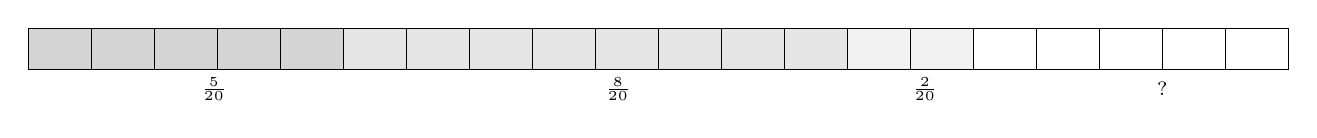
\begin{tikzpicture}[x=0.80cm, y=0.52cm, every node/.style={font=\scriptsize, text=black}]
    \foreach \i in {0,...,4}  { \fill[gray!34] (\i,0) rectangle (\i+1,1); }
    \foreach \i in {5,...,12} { \fill[gray!20] (\i,0) rectangle (\i+1,1); }
    \foreach \i in {13,14}    { \fill[gray!10] (\i,0) rectangle (\i+1,1); }
    \foreach \i in {0,...,19} { \draw[black, line width=0.65pt] (\i,0) rectangle (\i+1,1); }
    \node at (2.5,-0.48) {តន្ត្រីករ $\frac{5}{20}$};
    \node at (9.0,-0.48) {សិល្បករ $\frac{8}{20}$};
    \node at (14.0,-0.48) {របាំ $\frac{2}{20}$};
    \node at (17.5,-0.48) {\textbf{អ្នកនិពន្ធ $?$}};
  \end{tikzpicture}
  \end{center}
  \vspace{1pt}
  (១) ផលបូកប្រភាគក្រុមទាំងបី៖ $\dfrac{1}{4}+\dfrac{2}{5}+\dfrac{1}{10} = \dfrac{5 + \blank[0.7cm] + \blank[0.7cm]}{20} = \dfrac{\blank[0.8cm]}{20} = \blank[1.1cm]$ \;\en{|}\;
  (២) អ្នកនិពន្ធ៖ $1 - \blank[0.9cm] = \blank[1.1cm]$
\end{tcolorbox}

% --- E3 ---
\secbar{ផ្នែកទី២៖ សំយោគបញ្ញត្តិ \enbf{(E3)} និងធនាគារហេតុផល \enbf{B\&W} \cnum{1}\enbf{--}\cnum{5}}{សៀវភៅពុម្ព ទំ.៧–៨}

\begin{tabular}{|L{9.20cm}|L{9.20cm}|}
  \hline
  \textbf{១. រូបមន្តប្រមាណវិធីដក និងទំនាក់ទំនងសំខាន់ៗ៖}\par\vspace{3pt}
  $\bullet$ \textbf{ភាគបែងដូចគ្នា៖} $\dfrac{a}{b} - \dfrac{c}{b} = \dfrac{\blank[1.3cm]}{b}$ ($b\neq 0$)\par\vspace{3pt}
  $\bullet$ \textbf{ជាទូទៅ៖} $\dfrac{a}{b} - \dfrac{c}{d} = \dfrac{ad - \blank[0.9cm]}{bd}$ (ឬប្រើ \en{PPCM}$(b,d)$)\par\vspace{3pt}
  $\bullet$ \textbf{ប្ដូរដកជាបូកចំនួនផ្ទុយ៖} $\dfrac{a}{b} - \dfrac{c}{d} = \dfrac{a}{b} + \left(\blank[1.1cm]\right)$\par\vspace{3pt}
  $\bullet$ \textbf{ប្រយ័ត្ន៖} វិធីដក\textbf{គ្មាន}លក្ខណៈត្រឡប់ទេ ($\frac{a}{b}-\frac{c}{d} \neq \frac{c}{d}-\frac{a}{b}$)
  &
  \textbf{២. ធនាគារហេតុផល \en{B\&W} (\cnum{1}--\cnum{5})៖}\par\vspace{3pt}
  \cnum{1} តម្រូវភាគបែងរួមសិន ទើបយកភាគយកទី១ ដកភាគយកទី២ ។\par\vspace{3pt}
  \cnum{2} សោសញ្ញាដកពីរជាន់៖ $a - (-b) = a + b$ (ប្ដូរជាបូក) ។\par\vspace{3pt}
  \cnum{3} ដកថែមពីអវិជ្ជមាន៖ $-a - b = -(a+b)$ (រក្សាសញ្ញាដក) ។\par\vspace{3pt}
  \cnum{4} ចំនួនចម្រុះអវិជ្ជមាន៖ $-k\frac{r}{b} = -\frac{kb+r}{b}$ មុនបើកសោសញ្ញា ។\par\vspace{3pt}
  \cnum{5} ប្រភាគនៅសល់ពីទាំងមូល៖ យក $1 = \frac{b}{b}$ ដកផលបូកផ្នែកស្គាល់ ។ \\
  \hline
\end{tabular}

\vspace{5pt}
\begin{tcolorbox}[enhanced, sharp corners, colback=panelgray, colframe=black, boxrule=0.65pt, boxsep=1.5pt, top=2.5pt, bottom=2.5pt, left=5pt, right=5pt]
  \textbf{ប្រយ័ត្នអន្ទាក់៖} (១) $\dfrac{a}{b}-\dfrac{c}{d} \neq \dfrac{a-c}{b-d}$ ដាច់ខាត! \quad (២) $-\dfrac{5}{24}-\dfrac{7}{30} = -\dfrac{53}{120}$ \textbf{មិនមែន} $+\dfrac{53}{120}$ ឡើយ!
\end{tcolorbox}

\vspace{5pt}
\textbf{៣. លំហាត់ត្រួតពិនិត្យរហ័ស៖ គណនាផលដកចំនួនសនិទានដោយផ្ទាល់មាត់ និងដោយដៃ}

\vspace{3pt}
{\renewcommand{\arraystretch}{1.70}
\begin{tabular}{|C{4.40cm}|C{4.40cm}|C{4.40cm}|C{4.40cm}|}
  \hline
  \rowcolor{panelgray}
  $\frac{7}{9} - \frac{5}{9} = \blank[1.1cm]$ & $\frac{3}{7} - \frac{6}{7} = \blank[1.1cm]$ & $\frac{1}{2} - \left(-\frac{1}{2}\right) = \blank[1.0cm]$ & $1 - \frac{3}{8} = \blank[1.1cm]$ \\
  \hline
  $-\frac{2}{5} - \frac{3}{5} = \blank[1.1cm]$ & $\frac{9}{12} - \frac{2}{3} = \blank[1.1cm]$ & $0 - \left(-\frac{4}{11}\right) = \blank[1.0cm]$ & $1.5 - \frac{1}{2} = \blank[1.1cm]$ \\
  \hline
  $-\frac{4}{7} - \left(-\frac{4}{7}\right) = \blank[1.0cm]$ & $\frac{1}{4} - \frac{5}{8} = \blank[1.1cm]$ & $-1\frac{2}{5} = -\frac{\blank[0.7cm]}{5}$ & $2 - \frac{5}{3} = \blank[1.1cm]$ \\
  \hline
  $\frac{5}{6} - \frac{1}{6} = \blank[1.1cm]$ & $-\frac{1}{3} - \frac{2}{3} = \blank[1.1cm]$ & $-\frac{3}{10} - \left(-\frac{7}{10}\right) = \blank[0.9cm]$ & $1 - \frac{7}{12} = \blank[1.1cm]$ \\
  \hline
\end{tabular}}

\newpage

% ============================================================================
% ទំព័រទី ២៖ E4 លំហាត់គំរូ + E5 ប្រតិបត្តិ & វិនិច្ឆ័យ A-D + Exit + កិច្ចការផ្ទះ
% ============================================================================
\secbar{ផ្នែកទី៣៖ ពង្រីកចំណេះដឹងលើផលដកចំនួនចម្រុះ និងកន្សោមចម្រុះ \enbf{(E4 --} ទំ\enbf{.}៧ និងទំ\enbf{.}១២\enbf{)}}{រយៈពេល ១០ នាទី}

\textbf{លំហាត់ពង្រីកចំណេះដឹង៖} ចូរបំពេញជំហានគណនាខាងក្រោមដោយដៃ ព្រមទាំងបញ្ជាក់លេខហេតុផល \cnum{1}--\cnum{5}៖

{\renewcommand{\arraystretch}{1.54}
\begin{tabular}{|L{4.60cm}|L{9.20cm}|C{4.00cm}|}
  \hline
  \rowcolor{headgray}
  \textbf{ប្រធានលំហាត់ (ទំ.៧ និង ១២)} & \textbf{ដំណើរការគណនាដោយដៃតាមលំដាប់} & \textbf{ចម្លើយ និងហេតុផល} \\
  \hline
  \textbf{១. គំរូទី១ ខ (ទំ.៧)}\par\vspace{2pt}$\dfrac{9}{12} - \dfrac{2}{3}$ & $\text{\en{PPCM}}(12,3)=12 \implies \dfrac{9 - \blank[0.8cm]}{12}$ & $=\blank[1.4cm]$ (\cnum{1}) \\
  \hline
  \textbf{២. ចំនួនចម្រុះ (ទំ.១២ \#9ខ)}\par\vspace{2pt}$\left(-3\dfrac{1}{8}\right) - \left(-2\dfrac{5}{9}\right)$ & $=\dfrac{-\blank[0.8cm]}{8} + \dfrac{23}{9} = \dfrac{-225 + \blank[0.9cm]}{72}$ & $=\blank[1.4cm]$ (\cnum{4}, \cnum{2}) \\
  \hline
  \textbf{៣. បូក-ដកបីតួ (ទំ.១២ \#10ង)}\par\vspace{2pt}$-\dfrac{11}{8} + \dfrac{21}{4} - \dfrac{17}{16}$ & $\text{\en{PPCM}}(8,4,16)=16 \implies \dfrac{-22 + \blank[0.8cm] - 17}{16}$ & $=\blank[1.4cm]$ (\cnum{1}) \\
  \hline
  \textbf{៤. បំពេញឯកតាពេញ $1$}\par\vspace{2pt}$1 - \left(\dfrac{1}{3} + \dfrac{2}{9}\right)$ & $= 1 - \left(\dfrac{\blank[0.7cm] + 2}{9}\right) = \dfrac{9}{9} - \dfrac{\blank[0.7cm]}{9}$ & $=\blank[1.4cm]$ (\cnum{5}) \\
  \hline
\end{tabular}}

\vspace{5pt}
$\bullet$ \textbf{សំណួរឆ្លុះបញ្ចាំង \en{(EIA Looking-Back)}៖} ហេតុអ្វី $-\dfrac{5}{6}-\left(-\dfrac{7}{3}\right)$ ប្ដូរជាសញ្ញាបូក ឯ $-\dfrac{5}{24}-\dfrac{7}{30}$ មិនប្ដូរជាបូកទេ?\\
ចម្លើយ៖ ព្រោះ $-\dfrac{5}{24}-\dfrac{7}{30} = -\dfrac{5}{24} + \left(\blank[1.2cm]\right)$ គឺជាការបូកចំនួនអវិជ្ជមានពីរ (\cnum{3})!

% --- E5 ---
\secbar{ផ្នែកទី៤៖ វាយតម្លៃលទ្ធផលសិក្សា \enbf{(E5 --} ប្រតិបត្តិ ទំ\enbf{.}៨ \enbf{+} វិនិច្ឆ័យ \enbf{A--D +} សំបុត្រចេញ\enbf{)}}{រយៈពេល ១០ នាទី}

\textbf{ក. លំហាត់ប្រតិបត្តិ (សៀវភៅពុម្ព ទំ.៨ — ធ្វើជាដៃគូ រួចប្ដូរសន្លឹកផ្ទៀងផ្ទាត់ \en{Pause-Review})៖}

{\renewcommand{\arraystretch}{1.52}
\begin{tabular}{|L{8.90cm}|L{8.90cm}|}
  \hline
  \textbf{១) ប្រតិបត្តិ ក (ទំ.៨)៖}\par\vspace{3pt}
  $-\dfrac{5}{24} - \dfrac{7}{30} \quad (\text{\en{PPCM}}(24,30) = 120)$\par\vspace{3pt}
  $= \dfrac{-\blank[0.8cm] - \blank[0.8cm]}{120} = \blank[1.6cm]$ (\cnum{3})\par\vspace{3pt}
  $\bullet$ \textbf{បិទ \en{E1}៖} $-\dfrac{5}{6} - \left(-\dfrac{7}{3}\right) = \blank[1.4cm]$ (\cnum{2})
  &
  \textbf{២) ប្រតិបត្តិ ខ (ទំ.៨)៖}\par\vspace{3pt}
  $\dfrac{1}{15} - \dfrac{27}{50} \quad (\text{\en{PPCM}}(15,50) = 150)$\par\vspace{3pt}
  $= \dfrac{\blank[0.8cm] - \blank[0.8cm]}{150} = \blank[1.6cm]$ (\cnum{1})\par\vspace{3pt}
  $\bullet$ \textbf{ផ្ទៀងផ្ទាត់សញ្ញា៖} តើ $\frac{1}{15}$ តូចជាង $\frac{27}{50}$ មែនទេ? \chkbox\ មែន \;\chkbox\ ទេ \\
  \hline
\end{tabular}}

\vspace{5pt}
\textbf{ខ. គូសវង់ជុំវិញជម្រើសត្រឹមត្រូវតែ ១ គត់ ក្នុងចំណោម \en{A, B, C, D} រួចសរសេរលេខហេតុផល \cnum{1}--\cnum{5}៖}

{\renewcommand{\arraystretch}{1.44}
\begin{tabular}{|L{8.90cm}|L{8.90cm}|}
  \hline
  \textbf{ជម្រើស \en{A}៖} $\dfrac{3}{5} - \dfrac{7}{10} = \dfrac{7 - 6}{10} = \dfrac{1}{10}$ &
  \textbf{ជម្រើស \en{B}៖} $-\dfrac{5}{6} - \left(-\dfrac{7}{3}\right) = \dfrac{-5 + 14}{6} = \dfrac{3}{2}$ \\
  \hline
  \textbf{ជម្រើស \en{C}៖} $-\dfrac{5}{24} - \dfrac{7}{30} = +\dfrac{53}{120}$ &
  \textbf{ជម្រើស \en{D}៖} $\dfrac{9}{12} - \dfrac{2}{3} = \dfrac{9 - 2}{12 - 3} = \dfrac{7}{9}$ \\
  \hline
\end{tabular}}

\vspace{5pt}
\begin{tcolorbox}[enhanced, sharp corners, colback=panelgray, colframe=black, boxrule=0.75pt, boxsep=1.5pt, top=2.5pt, bottom=2.5pt, left=5pt, right=5pt]
  \textbf{សំបុត្រចេញពីថ្នាក់ (\en{Exit Ticket} — ៦០ វិនាទី)៖} បើកសោសញ្ញា រួចគណនាផលដក៖\\
  $-\dfrac{3}{8} - \left(-\dfrac{5}{4}\right) = \dfrac{-3}{8} + \blank[1.2cm] = \dfrac{-3 + \blank[0.8cm]}{8} = \blank[1.3cm]$ \quad (ហេតុផល៖ \blank[1.2cm])
\end{tcolorbox}

% --- កិច្ចការផ្ទះ ---
\secbar{ផ្នែកទី៥៖ កិច្ចការផ្ទះ \enbf{(}សៀវភៅពុម្ព ទំ\enbf{.}៨ និងទំ\enbf{.}១២\enbf{)} និងបណ្ដាំផ្ញើ}{ធ្វើក្នុងសៀវភៅកិច្ចការផ្ទះ}
$\bullet$ \textbf{លំហាត់ ១៖} គណនា រួចសម្រួល៖ ក) $\dfrac{7}{12}-\dfrac{5}{8}$ \quad ខ) $-\dfrac{3}{14}-\left(-\dfrac{5}{21}\right)$ \quad គ) $\left(-2\dfrac{1}{5}\right)-\left(-\dfrac{7}{9}\right)$\\
$\bullet$ \textbf{លំហាត់ ២៖} គ្រួសារមួយចំណាយប្រាក់ចំណូលលើម្ហូប $\frac{1}{2}$ និងទឹក-ភ្លើង $\frac{1}{10}$ ។ រកប្រភាគប្រាក់នៅសល់ \;\en{|}\; \textbf{អានមុន៖} ចំណុច \textbf{៤. ប្រមាណវិធីគុណ} (ទំ.៨–៩) ។

\end{document}
